\xchapter{Caracterização dos softwares científicos}
{Este capítulo apresenta a caracterização dos softwares científicos de análise
estática de código-fonte a partir da revisão estruturada.}
\label{caracterizacao-ferramentas}

Caracterizar os {\it softwares científicos} do domínio de aplicação de análise
estática de código-fonte publicados em conferências de engenharia de software
com objetivo de compreender como estão sendo publicados e mantidos, classificar
e explorar estes softwares entre as distintas categorias deste domínio de
aplicação.

%\section{Fundamentação teórica}

\section{Planejamento do experimento}

% # Scope [why?]
% ## Goal
% # Planning [how?]
% ## Context selection
% ## Hypothesis Formulation
% ## Variables selection
% ## Selection of subjects
% ## Experiment design
% ### Choice of experiment design
% ### General design principles
% ### Standard design types
% ## Instrumentation
% ## Validity evaluation
% # Operation
% # Analysis and Interpretation
% ## Teste de hipótese
%
%\section{Data collection procedure}
%
%\begin{itemize}
%  \item Revisão estruturada para busca e seleção de ferramentas a partir de artigos acadêmicos
%  \item Caracterização inicial das ferramentas, dimensões: Linguagem, Lançamentos, Tamanho, Experiência de usuário, Contexto
%  \item Caracterização final das ferramentas, dimensões: Entrada, Linguagens suportadas
%\end{itemize}

\subsection{Revisão estruturada}

A revisão estruturada é um processo disciplinado para busca e seleção de {\it
softwares científicos} de um domínio específico a partir de critérios bem
definidos, de forma que seja possível a reprodução do estudo por parte de
pesquisadores interessados.

A revisão estruturada difere da revisão e do mapeamento sistemático por ser um
processo mais simples e menos rígido, onde o resultado final é um conjunto de
softwares, enquanto no mapeamento ou na revisão sistemática há um esforço em
caracterizar os artigos analisados o mesmo não ocorre na revisão estruturada.

A revisão estruturada é organizada em três atividades de (1) busca de artigos
(definição das fontes, obtenção dos artigos nas fontes), (2) filtro (definição
de critérios de busca, definição de script de busca) e (3) seleção de artigos
com publicação de ferramentas. Estas atividades estão representadas na Figura
\ref{figura-revisao-estruturada}.

\begin{figure}[h]
  \center
  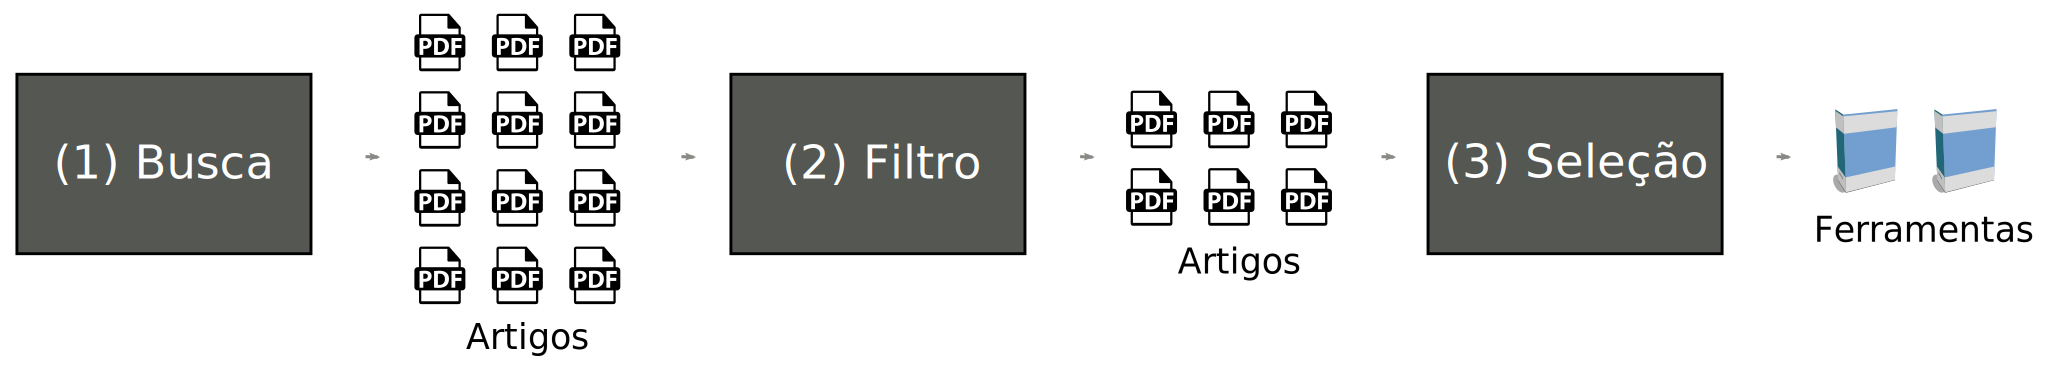
\includegraphics[scale=0.33]{imagens/revisao-estruturada.png}
  \caption{Atividades da revisão estruturada: (1) busca, (2) filtro e (3) seleção}
  \label{figura-revisao-estruturada}
\end{figure}

Na primeira atividade da revisão estruturada são definidas as fontes de busca,
estas fontes são conferências que abordam o tema de interesse do estudo, e que
apresentam um grande potencial de encontrar ferramentas de software
do domínio de aplicação desejado. Esta primeira atividade de busca deve
incluir o maior número possível de ediçoes das conferências selecionadas, para
cada edição são copiados localmente todos os artigos em PDF para posterior
filtro nas atividades subsequentes.

A segunda atividade da revisão estruturada realizada em cima de todo o conjunto
de artigos é um filtro automática que busca em todo o conteúdo dos artigos os
termos de interesse, estes termos devem ser pensados em relaçao ao domínio de aplicação
desejado, devem ser abrangentes a fim de evitar falsos negativos.

A terceira e última atividade da revisão estruturada é a seleção de artigos,
nela é identificado se cada artigo resulta, de fato, em publicação de {\it software científico}
do domínio de aplicação desejado. Esta seleção é feita a partir de uma
leitura superficial do artigo em busca de indícios de que o artigo publica uma
ferramenta do domínio em questão.

%O código-fonte da versão mais recente de cada
%uma destas ferramentas será copiado localmente para caracterização e análise
%através da coleta de suas métricas de código-fonte.

\subsection{Caracterização dos softwares científicos}
\label{caracterizacao}

Os {\it softwares científicos} de análise estática de código-fonte selecionados
na revisão estruturada serão avaliados inicialmente em relação à sua
disponibilidade visto a importância de tais artefatos para a divulgação do
conhecimento e para replicação dos resultados das pesquisas em engenharia de
software.

%, o artigo será lido em busca de informações onde obter uma
%cópia da ferramenta, o objetivo é avaliar a disponibilidade destas ferramentas.

\begin{description}

  \item {\it Disponibilidade - como a ferramenta foi publicada:}
    \begin{itemize}
      \item Artigo não indica onde obter a ferramenta
      \item Link para download da ferramenta offline
      \item Ferramenta disponivel para download (binários ou código-fonte)
    \end{itemize}

\end{description}

Em seguida serão caracterizadas a partir do trabalho de \citeonline{Novak2010},
neste estudo o autor propôe uma taxonomia e um conjunto de dimensões para
caracterização de ferramentas de análise estática. Um subconjunto destas
dimensões será utilizado na caracterização das ferramentas selecionadas
na revisão estruturada.

\begin{description}

  \item {\it Entrada - quais tipos de arquivos podem ser carregados na ferramenta:}
    \begin{itemize}
      \item Código-fonte - arquivos de código texto podem ser carregados
      \item Byte code - arquivos com Java Byte Code ou Microsoft
      \item Linguagem intermediária (MSIL) pode ser carregada
    \end{itemize}

  \item {\it Lançamentos ({\it Releases}) - quantos lançamentos por ano:}
    \begin{itemize}
      \item Frequentemente $>=$ 3 vezes ao ano - novas versões da ferramenta são lançadas 3 ou mais vezes por ano
      \item Ocasionalmente $<$ 3 vezes ao ano - novas versões da ferramenta são lançadas menos que 3 vezes ao ano
      \item Obsoleta 0 vezes ao ano - intervalo entre novos lançamentos é maior que 1 ano
    \end{itemize}

  \item {\it Linguagens suportadas - quais linguagens de programação a ferramenta suporta:}
    \begin{itemize}
      \item .NET - todas as linguagens compiladas em bibliotecas ou programas no framework .NET
      \item VB .NET - suporta VB.NET
      \item C\# - suporta C\#
      \item Java - suporta linguagem de programação Java
      \item C, C++ - suporta linguagem de programação C ou C++
    \end{itemize}

  \item {\it Disponibilidade - de que forma a ferramenta está disponível:}
    \begin{itemize}
      \item Código Aberto ({\it Open Source}) - a ferrament é livre e o código-fonte está disponível
      \item Grátis ({\it Free}) - a ferramenta é grátis mas o código-fonte não está disponível
      \item Comercial - a ferramenta está disponível mediante pagamento
    \end{itemize}

  \item {\it Experiência do usuário - de que forma a ferramenta pode ser usada, como é oferecida:}
    \begin{itemize}
      \item Integração com ambiente - como a ferramenta é integrada ao ambiente de trabalho
      \item Localização automática de erros no código - quando a ferramenta encontra um erro, ela leva ao local do erro
      \item Ajuda abrangente sobre falhas - se a ferramenta oferece ajuda na resolução de erros
      \item Interface de usuário - disponibilidade de uma interface de usuário
      \item Linha de comando - ela pode ser executada via linha de comando
      \item GUI - a ferramente pode ser executada em uma interface gráfica (GUI)
    \end{itemize}

  \item {\it Saída - representação dos resultados da ferramenta:}
    \begin{itemize}
      \item Arquivo texto - ferramenta pode apresentar resultados em arquivos texto
      \item Lista - ferramenta pode apresentar resultados numa interface de usuário customizada controlada em GUI
      \item Arquivo XML - ferramenta pode apresentar resultados em dados XML
      \item Arquivo HTML - ferramenta pode apresentar resultados em dados HTML
    \end{itemize}

\end{description}

As dimensões apresentada por \citeonline{Novak2010} não cobrem alguns aspectos
importantes percebidos ao longo deste estudo, assim novas dimensões serão utilizadas
em complemento às dimensões citadas acima.

\begin{description}

  \item {\it Linguagem de programação - em que linguagem de programação à ferramenta é escrita:}
    \begin{itemize}
      \item .NET
      \item VB .NET
      \item C\#
      \item Java
      \item C, C++
    \end{itemize}

%\end{description}
%
%Acrescentamos ainda novas opções que sentimos falta durante a caracterização das
%ferramentas, algumas dimensões de \cite{Novak2010} não apresentou opção necessária
%para caracterizar as ferramentas deste estudo, segue essas novas opções:
%
%\begin{description}

  \item {\it Saída - representação dos resultados da ferramenta:}
    \begin{itemize}
      \item Banco de dados - ferramenta pode armazenar resultados em banco de dados (relacional ou não-relacional)
    \end{itemize}

\end{description}

A fonte de informação para essa caracterização serão os artigos relacionados às
ferramentas, o código-fonte, documentos e site do projeto.

%Dimensões que
%envolvem coleta de métricas de código-fonte serão caracterizadas com o auxílio
%da ferramenta de análise de código-fonte Analizo, apresentada à seguir.

%\section{Seleção das ferramentas}

\section{Operação do experimento}

\subsection{Revisão estruturada}

Foi selecionada a conferência SCAM - {\it Source Code Analysis and Manipulation Working
Conference}\footnote{http://www.ieee-scam.org} e a conferência ASE - {\it Automated
Software Engineering}\footnote{http://ase-conferences.org}, por serem ambas
conferências com largo histórico de publicação sobre análise de programas.

A primeira atividade da revisão estruturada, busca, passa por todas as ediçoes
destas duas conferências até o ano de 2015, uma lista completa e o endereço de
cada edição onde os artigos foram obtidos está documentado no Apêndice
\ref{edicoes-conferencias}, lá é indicado o endereço da conferência nos
respectivos portais onde os artigos em PDF foram obtidos.

Esta atividade de busca resultou num total de 1879 artigos, 346 artigos do SCAM
e 1533 artigos do ASE, a Figura \ref{grafico-total-artigos} (a) apresenta um
gráfico com estes números.

\begin{figure}[H]
  \center
  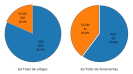
\includegraphics[scale=0.9]{imagens/total-artigos-e-ferramentas.png}
  \caption{Total de artigos e ferramentas por conferência (até o ano de 2015)}
  \label{grafico-total-artigos}
\end{figure}

A segunda atividade da revisão estruturada, filtro, realizada em cima deste conjunto
inicial de 1879 artigos é um filtro automático de busca que pesquisa em todos
os artigos os seguintes termos.

\begin{verbatim}
  "tool" OU "framework"; E
  "download" OU "available"; E
  "http" OU "ftp"; E
  "static analysis" OU "parser".
\end{verbatim}

Estes termos devem encontrar artigos com publicação de {\it softwares
científicos} do domínio de análise estática de código-fonte com disponibilidade
para {\it download}, seja binários ou código-fonte, o filtro realizado nesta
etapa no conjunto de 1879 artigos resultou em 436 artigos, deste total,
155 artigos da conferência SCAM e 281 da conferência ASE.

Estes 436 artigos com possível publicação de {\it software científico} de
análise estática de código-fonte são submetidos à terceira e última atividade
da revisão estruturada, seleção, nesta etapa cada artigo é lido, inicialmente
apenas introdução, resultados e conclusão com o objetivo de identificar se o
artigo publica {\it software científico} e indica onde obter uma cópia do
software. {\it Softwares científicos} que sejam mais abrangentes do que apenas
análise estática de código-fonte mas que contenham esta função em seu conjunto
também são selecionadas.

A atividade de seleção, última etapa da revisão estruturada, resultou em 103
artigos com publicação de {\it software científico} do domínio de aplicação de
análise estática de código-fonte, deste total 41 são da conferência
SCAM e 62 da conferência ASE, a Figura \ref{grafico-total-artigos} (b) e as
Figuras \ref{ferramentas-por-conferencia} (a) e (b) apresentam um resumo destes
números, as Tabelas \ref{artigos-do-scam} e \ref{artigos-do-ase} detalham os
resultados da revisão para cada edição das conferências analisadas.

\begin{figure}[h]
  \center
  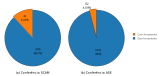
\includegraphics[scale=1]{imagens/ferramentas-por-conferencia.png}
  \caption{Total de artigos com ferramentas (até o ano de 2015)}
  \label{ferramentas-por-conferencia}
\end{figure}

\begin{table}[h]
\caption{Resultados da revisão estruturada para cada edição do SCAM}
\centering
\begin{tabular}{| l | c | c | c |}
\hline
Edição & (1) Busca & (2) Filtro & (3) Seleção \\
\hline
SCAM 2001 & 23    & 6         & 1           \\
SCAM 2002 & 18    & 6         & 5           \\
SCAM 2003 & 21    & 8         & 3           \\
SCAM 2004 & 17    & 3         & 1           \\
SCAM 2005 & 19    & 7         & 1           \\
SCAM 2006 & 22    & 10        & 7           \\
SCAM 2007 & 23    & 7         & 2           \\
SCAM 2008 & 29    & 14        & 2           \\
SCAM 2009 & 20    & 10        & -           \\
SCAM 2010 & 21    & 15        & 5           \\
SCAM 2011 & 21    & 10        & 2           \\
SCAM 2012 & 22    & 12        & 4           \\
SCAM 2013 & 24    & 13        & 2           \\
SCAM 2014 & 36    & 16        & 4           \\
SCAM 2015 & 30    & 18        & 2           \\
\hline
Total     & 346   & 155       & 41          \\
\hline
\end{tabular}
\label{artigos-do-scam}
\end{table}

\begin{table}[h]
\caption{Resultados da revisão estruturada para cada edição do ASE}
\centering
\begin{tabular}{| l | c | c | c |}
\hline
Edição & (1) Busca & (2) Filtro & (3) Seleção \\
\hline
ASE 1991 & 28    & -         & -           \\
ASE 1992 & 25    & -         & -           \\
ASE 1993 & 21    & -         & -           \\
ASE 1994 & 23    & -         & -           \\
ASE 1995 & 23    & -         & -           \\
ASE 1996 & 15    & -         & -           \\
ASE 1997 & 47    & 1         & -           \\
ASE 1998 & 44    & 4         & -           \\
ASE 1999 & 50    & -         & -           \\
ASE 2000 & 44    & 2         & -           \\
ASE 2001 & 68    & 7         & 2           \\
ASE 2002 & 46    & 5         & -           \\
ASE 2003 & 54    & 5         & 2           \\
ASE 2004 & 68    & 7         & -           \\
ASE 2005 & 79    & 9         & 1           \\
ASE 2006 & 61    & 12        & 2           \\
ASE 2007 & 102   & 19        & 5           \\
ASE 2008 & 90    & 18        & 5           \\
ASE 2009 & 89    & 19        & 11          \\
ASE 2010 & 87    & 20        & 3           \\
ASE 2011 & 112   & 28        & 5           \\
ASE 2012 & 68    & 16        & 5           \\
ASE 2013 & 90    & 28        & 7           \\
ASE 2014 & 100   & 39        & 7           \\
ASE 2015 & 99    & 42        & 7           \\
\hline
Total    & 1533  & 281       & 62          \\
\hline
\end{tabular}
\label{artigos-do-ase}
\end{table}

\subsection{Caracterização dos softwares científicos}

A seção à seguir traz uma caracterização inicial das ferramentas segundo às
categorias citadas anteriormente.

\begin{figure}[h]
  \center
  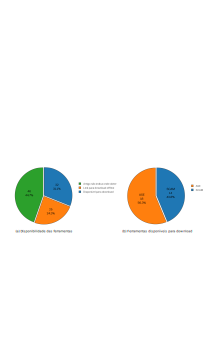
\includegraphics[scale=0.85]{imagens/ferramentas-disponiveis.png}
  \caption{Ferramentas disponíveis para download (até o ano de 2015)}
  \label{ferramentas-disponiveis}
\end{figure}

As informações foram obtidas de forma manual lendo a documentação da ferramenta
junto ao código-fonte ou no site da mesma.  Ao final desde capítulo a tabela
\ref{total-de-ferramentas} apresenta um resumo da caracterização feita.

\begin{table}[h]
{\scriptsize
\caption{Resumo das ferramentas selecionadas}
\centering
\begin{tabular}{| l | l | l | l |}
  \hline
  Ferramenta     & Descrição                            & Ferramenta       & Descrição                            \\
  \hline
  2LS            & análise de terminação de programas   & JstereoCode      & detecção de esteriótipos Java        \\
  AccessAnalysis & cálculo de métricas IGAT e IGAM      & JSysDG           & construção de grafo de dependência   \\
  ADiMat         & transformação source-to-source       & Jtop             & gestão de casos de teste             \\
  AGENDA         & teste de banco de dados relacional   & Kiasan/Bogor     & verificação de modelos               \\
  AMNESIA        & detecção de ataques SQL injection    & LIBCROOS         & localização de bugs                  \\
  AMOEBA         & correção de erros de modelagem       & Loopfrog         & verificação de modelos               \\
  APIExample     & documentação de API Java             & Lotrack          & análise estática de configuração     \\
  BEG            & verificação de modelos Java          & MAGIC            & program slicing                      \\
  BEST           & predição de violação de concorrência & MemSafe          & detecta violação de acesso a memória \\
  CAWDOR         & defesa e deteção de worms            & MPAnalyzer       & análise de padrões                   \\
  CBFA           & detecção de concerns                 & MSP              & criação de modelo de acesso a memória \\
  ccJava         & linguagem orientada a aspectos       & mygcc            & verificação de programas C           \\
  CIVL           & verificação de programa concorrente  & Parfait          & localização de bugs                  \\
  ClassSplitter  & particionamento de classes           & PARSEWeb         & sugestão de uso de código e bibliotecas \\
  CodeBoost      & transformação source-to-source C++   & PAT              & ambiente de teste automático         \\
  CodeHow        & busca e pesquisa em código           & ProgramCutter    & particionamento automático           \\
  composite      & verificação de modelos               & protopurity      & análise de impacto                   \\
  CONBOL         & criação automática de teste          & Pseudogen        & transformação source-to-pseudo-source \\
  COPES          & detecção de falhas de permissão      & PtrTracker       & detecção de bugs                     \\
  CPA+           & análise configurável de programa     & PtYasm           & verificação de modelos               \\
  CPPCHECKER     & detecção de inconsistência em macros & PuMoC            & verificação de modelos               \\
  CSeq           & transformação source-to-source       & PYTHIA           & criação automática de casos de teste \\
  DDVerify       & checagem de modelos                  & ReAssert         & localização de falhas em testes      \\
  Decor          & detecção de defeitos de design       & Relda            & localização de vazamento de recurso  \\
  Derailer       & localização de falhas de segurança   & Rêve             & verificação de regressão             \\
  Diagnosys      & construção de interfaces de debug    & ReWeb            & refatoração de aplicações Web        \\
  DMS            & transformação de programas           & RRFinder         & mineração de liberação de recursos   \\
  Doc2Spec       & inferência de especificação de API   & SAFEWApp         & ???                                  \\
  DOMPLETION     & sugestão de código javascript        & Sapid/XML        & ???                                  \\
  Drails         & detecção de erros de runtime         & SCATR            & mapeamento baseado em código         \\
  EJB            & criação de diagramas de sequência    & Scoria           & localização de violação arquitetural \\
  ELAN           & inspeção de resultados de defeitos   & Smack            & checagem de memória                  \\
  EMBER          & cálculo de métricas de código-fonte  & SonarQubePlug-in & ???                                  \\
  e-munity       & verificação de segurança             & SPARTA           & segurança e detecção de malwares     \\
  error-prone    & localização de bugs                  & srcML            & transformação source-to-source       \\
  ESBMC          & verificação de modelos               & SUDS             & detecção de bugs                     \\
  ETXL           & transformação de código              & SWAT             & teste automático para aplicação web  \\
  FaultBuster    & refatoração de code smells           & SymCrash         & geração de casos de teste            \\
  Flowgen        & criação de grafos UML                & TACLE            & type-analysis e visualizaçao de call-graph \\
  GASR           & query lógica para AspectJ            & TEBA             & ???                                  \\
  Goanna         & checagem de modelos                  & Templar          & visualização de código               \\
  GRT            & geração automática de testes         & TestEra          & geração automática de testes         \\
  GUIZMO         & inferência de layout                 & Tikanga          & detecção de violação                 \\
  GumTree        & análise e comparação de mudanças     & UMGAR            & geração de modelos UML               \\
  HaRe           & refatoração de código funcional      & VADA             & análise de dependencia de variáveis  \\
  iMaus          & detecção de código duplicado         & Vdiff            & visualização de diferença de código  \\
  Impendulo      & ???                                  & WAIVE+           & ???                                  \\
  Indus          & biblioteca de program slicing        & WALA             & análise de {\it bytecode} Java       \\
  ISIS4J         & identificação de concerns            & Wrangler         & refatoração de código Erlang         \\
  JastAdd        & descrição e gramática de atributos   & X-DEVELOP        & refatoração                          \\
  JFlow          & transformação source-to-source       & XOgastan         & transformação source-to-source       \\
  \hline
\end{tabular}
\label{resumo-de-ferramentas}
}
\end{table}

% \subsection{AccessAnalysis}
% 
% disponível em \url{http://accessanalysis.sourceforge.net}. O código-fonte
% utilizado em nosso estudo obtido no site da ferramenta foi o
% \texttt{AccessAnalysis-1.2-src.zip}.
% 
% \subsection{Kiasan/Bogor}
% 
% Ferramenta de verificação de modelo disponível em
% \url{http://bogor.projects.cs.ksu.edu/manual}. O código-fonte utilizado em
% nosso estudo obtido no site da ferramenta foi o
% \texttt{bogor-src-1.2.20061023.1.zip}.
% 
% Não possui número suficiente de releases para ser usado na análise evolutiva.
% 
% \subsection{composite}
% 
% Ferramenta de verificação de modelo disponível em
% \url{http://www.cs.ucsb.edu/~bultan/composite/}. O código-fonte utilizado em
% nosso estudo obtido no site da ferramenta foi o \texttt{composite-0.4.tar.gz}.
% 
% \subsection{CSeq}
% 
% Ferramenta de transformação {\it source-to-source} para programas C
% concorrentes disponível em
% \url{http://users.ecs.soton.ac.uk/gp4/cseq/files/cseq-0.5.zip}. O código-fonte
% utilizado em nosso estudo obtido no site da ferramenta foi o
% \texttt{cseq-0.5.zip}.
% 
% \subsection{EJB}
% 
% Ferramenta de análise estática para criação de diagramas de sequência
% disponível em
% \url{https://www.dropbox.com/s/glhg8any43lccgm/EJB.zip}.
% 
% \subsection{error-prone}
% 
% Ferramenta de localização de bugs em código Java construída em cima do
% compilador {\it javac} disponível em
% \url{http://code.google.com/p/error-prone}. O código-fonte utilizado em nosso
% estudo obtido no site da ferramenta foi o \texttt{error-prone-2.0.9.tar.gz}.
% 
% \subsection{GUIZMO}
% 
% Ferramenta de inferência de layout disponível em
% \url{http://modelum.es/trac/guizmo/}, plugin Eclipse. O código-fonte
% utilizado em nosso estudo obtido no site da ferramenta foi o
% \texttt{guizmo-master.zip}. Aceita como entrada um formato baseado em
% XML\footnote{\url{http://wireframesketcher.com/help/xmlformat.html}} e gera
% código GUI em Java Swing / ZK.
% 
% \subsection{GumTree}
% 
% Ferramenta de análise de código-fonte e comparação de mudanças
% disponível em \url{https://github.com/jrfaller/gumtree}. O
% código-fonte utilizado em nosso estudo obtido no site da ferramenta foi o
% \texttt{gumtree-2.0.0.tar.gz}.
% 
% \subsection{Indus}
% 
% Biblioteca de {\it program
% slicing}\footnote{http://en.wikipedia.org/wiki/Program\_slicing} Java disponível em
% \url{http://indus.projects.cs.ksu.edu}. O projeto está organizado em três
% módulos, os seguintes arquivos, contendo o código-fonte dos três módulos,
% foram copiados localmente para análise:
% \texttt{indus.indus-src-20091220.zip},
% \texttt{indus.javaslicer-src-20091220.zip} e
% \texttt{indus.staticanalyses-src-20070305.zip}.
% 
% Não possui número suficiente de releases para ser usado na análise evolutiva.
% 
% \subsection{JastAdd}
% 
% Sistema para análise de código-fonte através da descrição de
% atributos via gramática de atributos (AG) disponível em \url{http://jastadd.cs.lth.se/web}. O código-fonte
% utilizado em nosso estudo obtido no site da ferramenta foi o
% \texttt{jastadd2-src.zip}.
% 
% \subsection{JFlow}
% 
% Ferramenta de transformação {\it source-to-source} disponível em
% \url{http://vazexqi.github.io/JFlow/}. O código-fonte
% utilizado em nosso estudo obtido no site da ferramenta foi o
% \texttt{vazexqi-JFlow-7cd7eaf.tar.gz}.
% 
% \subsection{Lotrack}
% 
% Ferramenta de análise estática de configuração disponível em
% \url{https://github.com/MaxLillack/Lotrack}. O código-fonte utilizado em nosso
% estudo obtido no site da ferramenta foi o \texttt{Lotrack-master.zip}.
% 
% Não possui número suficiente de releases para ser usado na análise evolutiva.
% 
% \subsection{MPAnalyzer}
% 
% Ferramenta de análise de padrões disponível em
% \url{https://github.com/YoshikiHigo/MPAnalyzer}. O código-fonte utilizado em
% nosso estudo obtido no site da ferramenta foi o \texttt{MPAnalyzer-master.zip}.
% 
% \subsection{PtYasm}
% 
% Ferramenta de verificação de modelo disponível em
% \url{www.cs.toronto.edu/~tomhart/ptyasm}. O código-fonte
% utilizado em nosso estudo obtido no site da ferramenta foi o
% \texttt{ptyasm.april2008.tgz}.
% 
% Não possui número suficiente de releases para ser usado na análise evolutiva.
% 
% \subsection{ReAssert}
% 
% Ferramenta de localização de falhas em testes e refatoração
% desenvolvido como plugin Ecipse disponível em
% \url{http://mir.cs.illinois.edu/reassert}. O código-fonte utilizado em nosso
% estudo obtido no site da ferramenta foi o \texttt{ReAssert\_0.4.1-src.zip}.
% 
% \subsection{Sonar Qube Plug-in}
% 
% Plugin para o SourceMeter que extende a análise de
% código Java com o uso do SonarQube disponível em:
% \url{http://github.com/FrontEndART/SonarQube-plug-in}. O código-fonte
% utilizado em nosso estudo obtido no site da ferramenta foi o
% \texttt{SonarQube-plug-in-master.zip}.
% 
% \subsection{SPARTA}
% 
% Ferramenta de análise estática de segurança pra detecção de {\it
% malware} disponível em
% \url{http://types.cs.washington.edu/sparta/}. O código-fonte utilizado em nosso
% estudo obtido no site da ferramenta foi o \texttt{sparta-sparta-1.0.2.tar.gz}.
% 
% \subsection{srcML}
% 
% Formato texto para representação de código-fonte e um conjunto de
% ferramentas de transformação {\it source-to-source} disponível em
% \url{http://www.sdml.info/projects/srcml/trunk}\footnote{este endereço
% retornou "not found" em contato com os autores por email indicaram que o
% projeto foi movido para http://www.srcML.org}. O código-fonte utilizado em
% nosso estudo obtido no site da ferramenta foi o \texttt{srcML-src.tar.gz}.
% 
% Não possui número suficiente de releases para ser usado na análise evolutiva.
% 
% \subsection{TACLE}
% 
% Plugin do Eclipse para análise de tipo ({\it Type Analysis}) e
% construção de visualizaçao de grafos de chamada ({\it Call Graph}) disponível em
% \url{http://presto.cse.ohio-state.edu/tacle}\footnote{este link está
% indisponível, por email os autores indicaram o endereço
% http://web.cse.ohio-state.edu/~rountev/presto/tacle/TACLE\_Download/tacle.html}.
% O código-fonte utilizado em nosso estudo obtido no site da ferramenta foi o
% \texttt{tacle\_1\_2\_1\_src.zip}.
% 
% \subsection{WALA}
% 
% Ferramenta de análise estática para {\it bytecode} Java disponível em
% \url{http://wala.sourceforge.net/wiki/index.php/Main_Page}. O código-fonte
% utilizado em nosso estudo obtido no site da ferramenta foi o
% \texttt{WALA-R\_1.3.8.tar.gz}.
% 
% Ferramenta selecionada para análise evolutiva, possui muitos releases e tem tamanho
% em número de classes na média.
% 
% \subsection{Closure Compiler}
% 
% Compilador que traduz código JavaScript em outro
% JavaScript melhor e mais otimizado, está disponível em
% \url{https://developers.google.com/closure/compiler}\footnote{O código fonte do
% Closure Compiler pode ser obtido em:
% http://github.com/google/closure-compiler} e foi utilizado em nosso estudo o
% seguinte lançamento
% \texttt{closure-compiler-closure-compiler-parent-v20160619.tar.gz}.
% 
% Ferramenta selecionada para análise evolutiva, possui muitos releases e tem tamanho
% em número de classes na média.
% 
% \subsection{Cppcheck}
% 
% Ferramenta de análise estática de código C/C++ para checagem de vazamento de
% memória, erros de alocação, entre outras falhas. Disponível em
% \url{http://sourceforge.net/projects/cppcheck}. Em nosso estudo utilizamos o
% código em \texttt{cppcheck-1.72.tar.bz2}.
% 
% \subsection{CQual}
% 
% Ferramenta de análise de typo ({\it type-based analysis}) que fornece um
% mecanismo leve e prático para especificação e verificação de propriedades de
% programas C. Disponível em \url{http://www.cs.umd.edu/~jfoster/cqual}. Em
% nosso estudo utilizamos o código em \texttt{cqual-0.981.tar.gz}.
% 
% \subsection{FindBugs}
% 
% Uma ferramenta para localização de bugs em código Java disponível em
% \url{http://findbugs.sourceforge.net}. Em nosso estudo utilizamos o código em
% \texttt{findbugs-3.0.1-source.zip}.
% 
% Ferramenta selecionada para análise evolutiva, possui muitos releases e tem tamanho
% em número de classes na média.
% 
% \subsection{FindSecurityBugs}
% 
% Plugin do FindBugs para auditoria de segurança em aplicações web Java,
% disponível em \url{http://find-sec-bugs.github.io}. O código-fonte utilizado
% em nosso estudo obtido no site da ferramenta foi o
% \texttt{findsecbugs-plugin-1.4.5-sources.jar}.
% 
% \subsection{Jlint}
% 
% Uma ferramenta para verificaçao de código Java em busca de bugs,
% inconsistências e problemas de sincronização disponível em
% \url{http://sourceforge.net/projects/jlint}.  O código-fonte utilizado em
% nosso estudo obtido no site da ferramenta foi o \texttt{jlint-3.1.2.zip}.
% 
% \subsection{Pixy}
% 
% Ferramenta de análise estática de código PHP para verificação de
% vulnerabilidades de segurança. Disponível em
% \url{http://github.com/oliverklee/pixy}. O código-fonte utilizado em nosso
% estudo obtido no site da ferramenta foi o \texttt{pixy-master.zip}.
% 
% \subsection{PMD}
% 
% Ferramenta de análise de código-fonte para localização falhas comuns de
% programação com suporte a várias linguagens, disponível em
% \url{http://pmd.github.io}. O código-fonte utilizado em nosso estudo obtido
% no site da ferramenta foi o \texttt{pmd-src-5.4.1.zip}.
% 
% Ferramenta selecionada para análise evolutiva, possui muitos releases e tem tamanho
% em número de classes na média.
% 
% \subsection{RATS}
% 
% Ferramenta de análise estática para auditoria de segurança 
% de códigos C, C++, Perl, PHP e Python disponível em
% \url{http://code.google.com/archive/p/rough-auditing-tool-for-security}. O
% código-fonte utilizado em nosso estudo obtido no site da ferramenta foi o
% \texttt{rats-2.4.tgz}.
% 
% \subsection{Smatch}
% 
% Ferramenta de análise estática para detecção de erros no Kernel disponível em
% \url{http://smatch.sourceforge.net}. O código-fonte utilizado em nosso estudo
% obtido no site da ferramenta foi o \texttt{smatch.git}.
% 
% \subsection{Splint}
% 
% Ferramenta para verificação de programas em C por vulnerabilidades de segurança e
% erros de código. Disponível em \url{http://www.splint.org}. O código-fonte
% utilizado em nosso estudo obtido no site da ferramenta foi o
% \texttt{splint-3.1.2.src.tgz}.
% 
% Não possui número suficiente de releases para ser usado na análise evolutiva.
% 
% \subsection{UNO}
% 
% Uma ferramenta de análise de código-fonte C para detecção de defeitos.
% Disponível em \url{http://spinroot.com/uno}. O código-fonte utilizado em nosso
% estudo obtido no site da ferramenta foi o \texttt{uno\_v213.tar.gz}.
% 
% \subsection{WAP}
% 
% Ferramenta para análise estática de código-fonte PHP e mineraçao de dados para
% detectar e corrigir vulnerabilidades em aplicações web. Disponível em
% \url{http://awap.sourceforge.net}. O código-fonte utilizado em nosso estudo
% obtido no site da ferramenta foi o \texttt{wap-2.1.tar.gz}.

\section{Conclusões}

% analise e interpretação

De forma que somando as ferramentas selecionadas na academia e na indústria
temos um total de 34 ferramentas, 14 da indústria e 20 da academia.  A Tabela
\ref{total-de-ferramentas} resume este total trazendo o nome de cada ferramenta
e algumas de suas características, a caracterização completa está documentado
no arquivo {\it
ferramentas-e-metricas.ods}\footnote{https://github.com/joenio/dissertacao-ufba-2016/blob/master/dataset/ferramentas-e-metricas.ods}
disponível no repositório desta dissertação.

\begin{table}[H]
  \caption{Resumo da caracterização das ferramentas}
  \centering
  \begin{tabular}{| c | l | l | c | l | l |}
    \hline
    \# & Ferramentas da indústria & Linguagem & Classes & Lançamentos \\
    \hline
    21 & Clang Static Analyzer    & C++   & ?     & Frequentemente \\
    22 & Closure Compiler         & Java  & 1842  & Frequentemente \\
    23 & Cppcheck                 & C++   & 338   & Frequentemente \\
    24 & CQual                    & C     & 78    & Obsoleta       \\
    25 & FindBugs                 & Java  & 1486  & Ocasionalmente \\
    26 & FindSecurityBugs         & Java  & 91    & Frequentemente \\
    27 & Jlint                    & C++   & 44    & Obsoleta       \\
    28 & Pixy                     & Java  & 229   & Obsoleta       \\
    29 & PMD                      & Java  & 1340  & Frequentemente \\
    30 & RATS                     & C     & 19    & Obsoleta       \\
    31 & Smatch                   & C     & 483   & Ocasionalmente \\
    32 & Splint                   & C     & 681   & Obsoleta       \\
    33 & UNO                      & C     & 19    & Obsoleta       \\
    34 & WAP                      & Java  & 338   & Frequentemente \\
    \hline
  \end{tabular}
  \label{total-de-ferramentas}
\end{table}

% documentar onde os dados, fontes, etc podem ser encontrados:

% os artigos foram documentados e estão disponíveis num arquivo externo
% {\it artigos.ods}\footnote{http://github.com/joenio/dissertacao-ufba-2016/blob/master/revisao-estruturada/artigos.ods}.
%
%com o auxílio do script
%{\it
%filter}\footnote{http://github.com/joenio/dissertacao-ufba-2016/blob/master/revisao-estruturada/filter}
%escrito especialmente para este estudo. 
%
%atividade (2) da revisao estruturada:
%Os artigos selecionados nesta atividade
%estão documentados no arquivo {\it artigos.ods} indicados na coluna ``Filtro(2)''
%quando for o caso.
